\chapter{Perancangan}
\label{chap:perancangan}

Pada bab ini akan dijelaskan mengenai perancangan kelas beserta deskripsi kelas dan fungsinya, serta perancangan antarmuka.

\section{Perancangan Kelas}
\label{perancanganKelas}

Diagram kelas secara keseluruhan dapat dilihat pada gambar \ref{fig:4_class_diagram}, dimana ~terdapat ~\textit{package screensaver} yang didalamnya terdapat \textit{package} siakad (Gambar \ref{fig:4_class_diagram_siakad}), dan \textit{package} studentportal (Gambar \ref{fig:4_class_diagram_stupor}).
Penjelasan mengenai kelas, \textit{method}, dan atribut jsoup terdapat pada bagian \ref{sec:jsoup}.
Penjelasan mengenai kelas, \textit{method}, dan atribut JavaFX serta FXML terdapat pada bagian \ref{sec:javafxfxml}. Penjelasan mengenai kelas, \textit{method}, dan atribut SIAModels terdapat pada bagian \ref{sec:siamodels}. 

\begin{figure}[h]
	\centering
	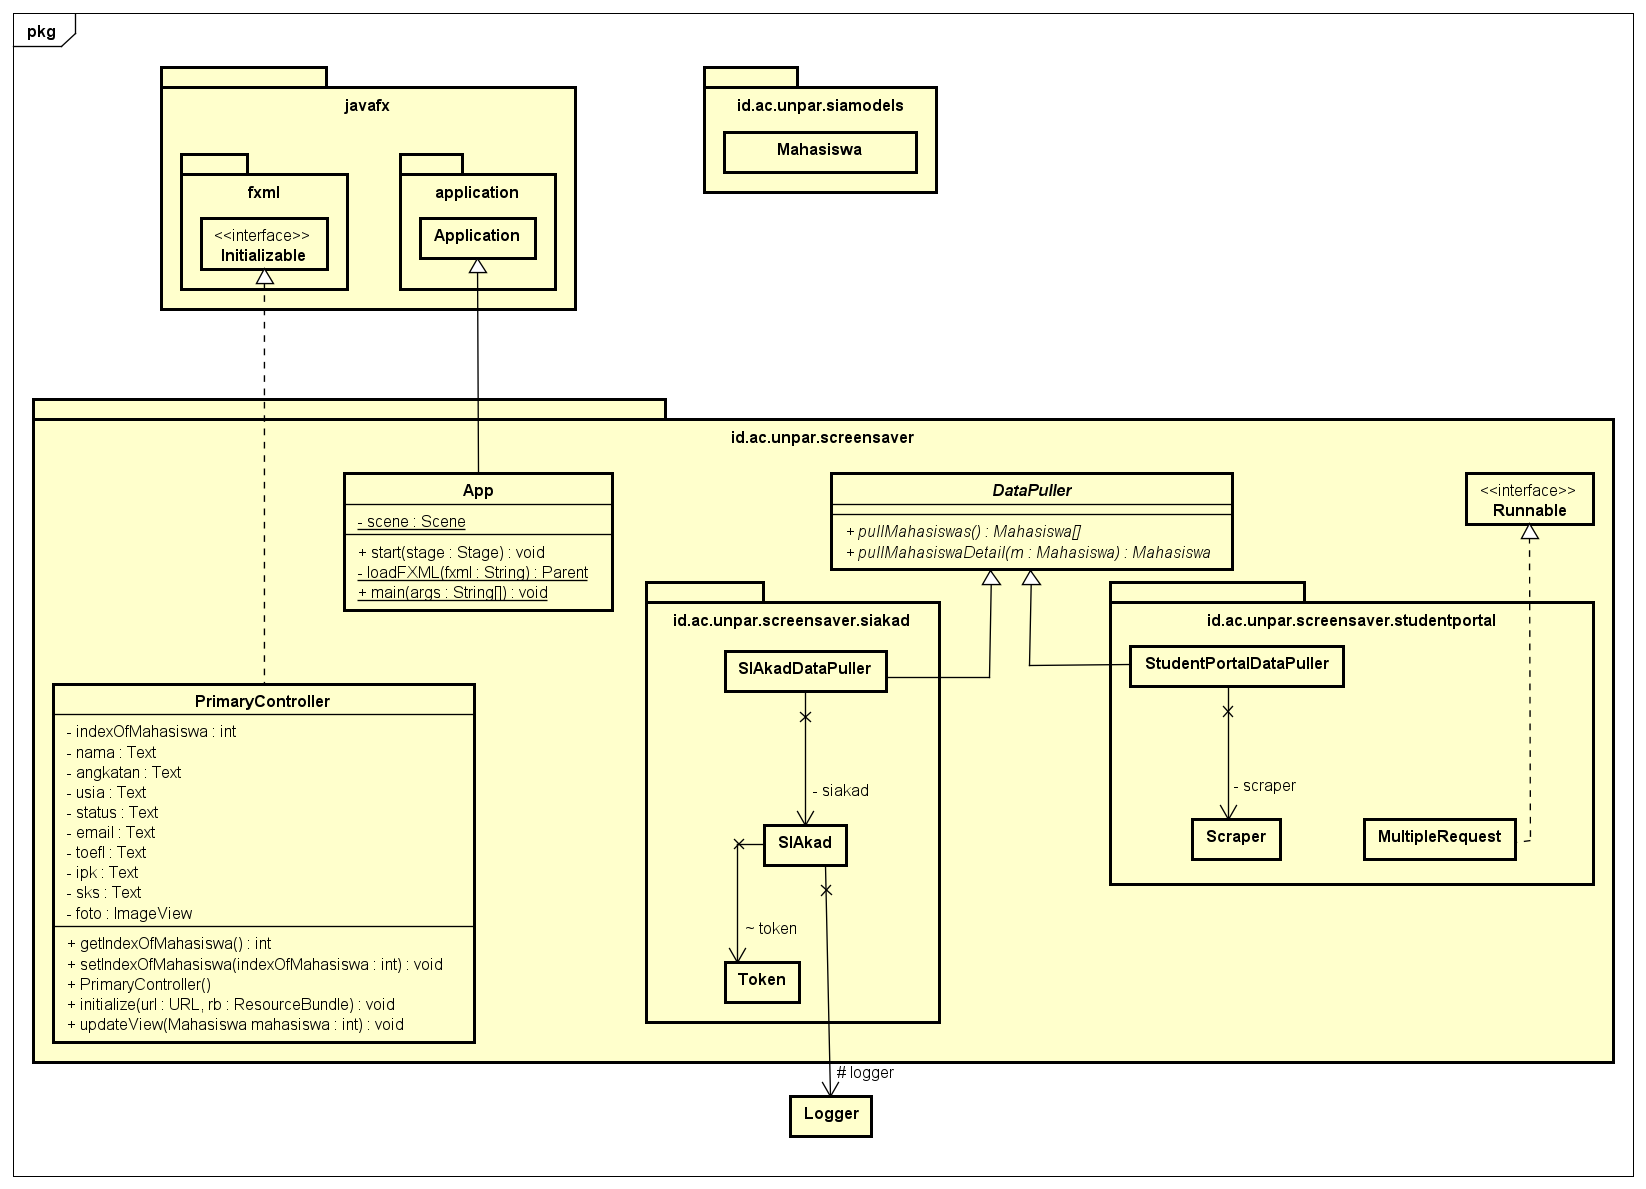
\includegraphics[scale=0.39]{Gambar/ClassDiagram.png}
	\caption{Diagram Kelas Keseluruhan}
	\label{fig:4_class_diagram}
\end{figure}

\begin{figure}[h]
	\centering
	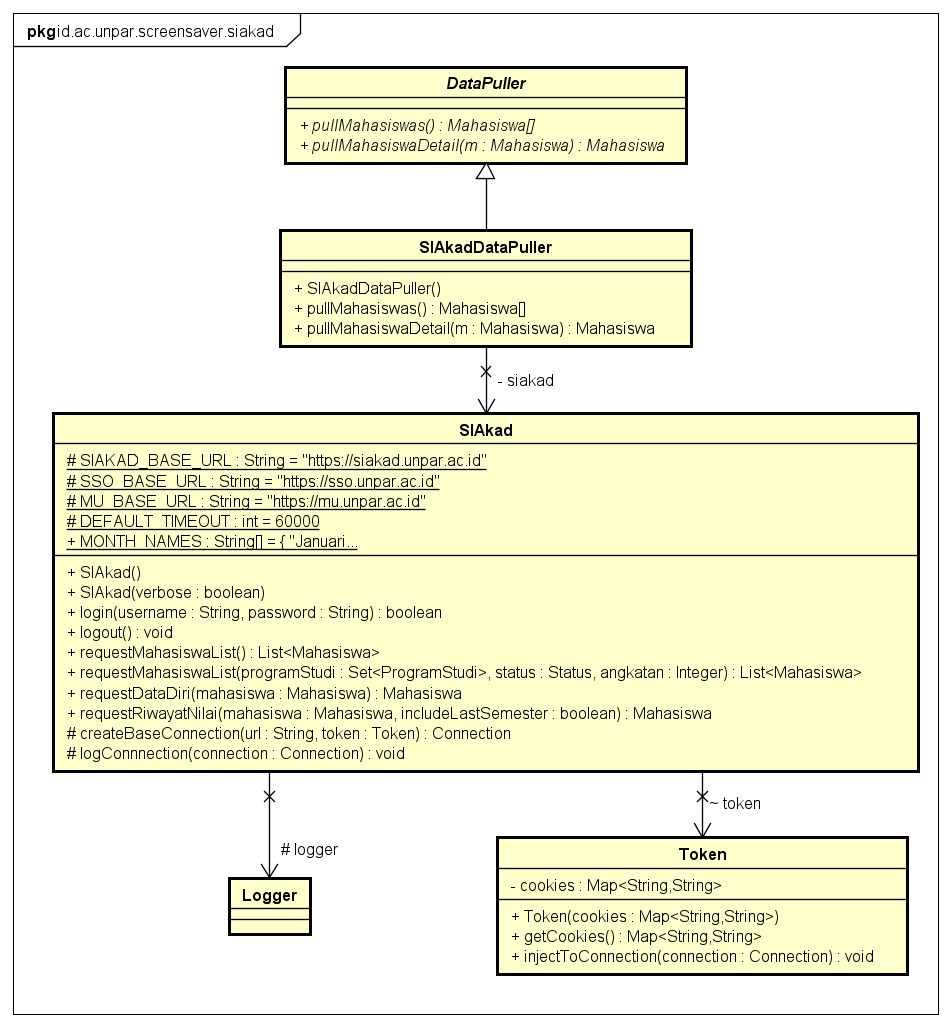
\includegraphics[scale=0.45]{Gambar/ClassDiagram_siakad.png}
	\caption{Diagram Kelas SIAKAD}
	\label{fig:4_class_diagram_siakad}
\end{figure}

\begin{figure}[h]
	\centering
	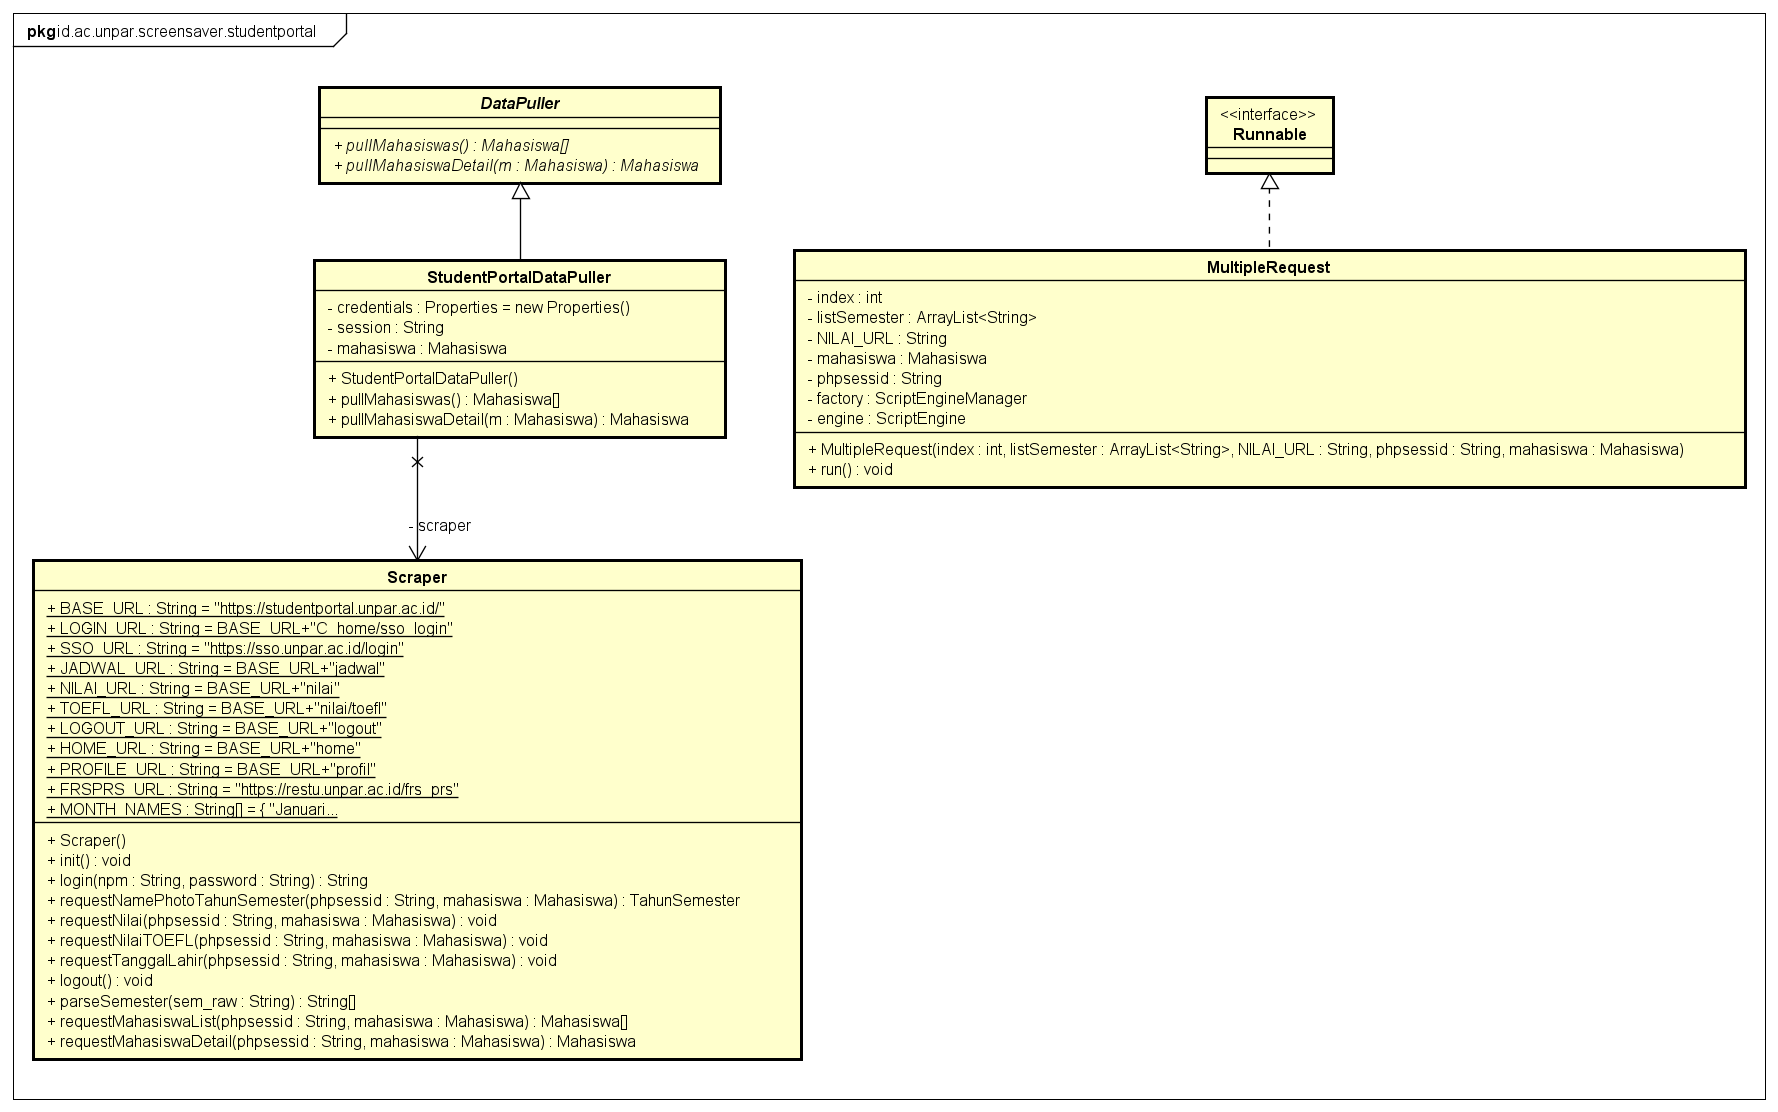
\includegraphics[scale=0.34]{Gambar/ClassDiagram_stupor.png}
	\caption{Diagram Kelas Studentportal}
	\label{fig:4_class_diagram_stupor}
\end{figure}

Penjelasan mengenai kelas, \textit{method}, dan atribut pada \textit{package screensaver} adalah sebagai berikut:
\begin{enumerate}

\item{App}\\
Kelas ini merupakan turunan dari kelas Application \ref{application}. Atribut yang dimiliki kelas ini adalah sebagai berikut:
\begin{itemize}
    \item \texttt{private static Scene scene:} menyimpan objek \texttt{Scene}.
\end{itemize}
\textit{Method} yang dimiliki kelas ini adalah sebagai berikut:
\begin{itemize}
    \item \texttt{public void start(Stage stage)}\\
    Berfungsi untuk menampilkan \texttt{Stage} dengan \texttt{Scene} yang digunakan.\\
    \textbf{Parameter:}
	\begin{itemize}
		\item \texttt{stage:} \textit{stage} utama untuk aplikasi ini.
	\end{itemize}
    \item \texttt{private static Parent loadFXML(String fxml)}\\
    Berfungsi untuk memuat hierarki objek dari dokumen FXML.\\
    \textbf{Parameter:}
	\begin{itemize}
		\item \texttt{fxml:} dokumen fxml.
	\end{itemize}
	\textbf{Kembalian:} hierarki objek dari dokumen FXML.
    \item \texttt{public static void main(String[] args)}\\
    Berfungsi untuk memanggil \textit{method} \texttt{launch()} pada kelas \texttt{Application}.
\end{itemize}

\item{PrimaryController}\\
Kelas ini mengimplementasikan kelas \textit{interface Initializable} \ref{fxml}. Atribut yang dimiliki kelas ini adalah sebagai berikut:
\begin{itemize}
    \item \texttt{private int indexOfMahasiswa:} menyimpan indeks mahasiswa yang akan ditampilkan pada \textit{screensaver}.
    \item \texttt{private Text nama:} menyimpan objek \texttt{Text} yang digunakan untuk keterangan nama mahasiswa.
    \item \texttt{private Text angkatan:} menyimpan objek \texttt{Text} yang digunakan untuk keterangan angkatan mahasiswa.
    \item \texttt{private Text usia:} menyimpan objek \texttt{Text} yang digunakan untuk keterangan usia mahasiswa.
    \item \texttt{private Text status:} menyimpan objek \texttt{Text} yang digunakan untuk keterangan status mahasiswa.
    \item \texttt{private Text email:} menyimpan objek \texttt{Text} yang digunakan untuk keterangan \textit{email} mahasiswa.
    \item \texttt{private Text toefl:} menyimpan objek \texttt{Text} yang digunakan untuk keterangan nilai TOEFL mahasiswa.
    \item \texttt{private Text ipk:} menyimpan objek \texttt{Text} yang digunakan untuk keterangan IPK mahasiswa.
    \item \texttt{private Text sks:} menyimpan objek \texttt{Text} yang digunakan untuk keterangan SKS mahasiswa.
    \item \texttt{private ImageView foto:} menyimpan objek \texttt{ImageView} yang digunakan untuk foto mahasiswa.
\end{itemize}
\textit{Method} yang dimiliki kelas ini adalah sebagai berikut:
\begin{itemize}
    \item \texttt{public int getIndexOfMahasiswa()}\\
    Berfungsi untuk mengambil indeks mahasiswa.\\
	\textbf{Kembalian:} indeks mahasiswa.
    \item \texttt{public void setIndexOfMahasiswa(int indexOfMahasiswa)}\\
    Berfungsi untuk menyimpan indeks mahasiswa.\\
    \textbf{Parameter:}
	\begin{itemize}
		\item \texttt{indexOfMahasiswa:} indeks mahasiswa.
	\end{itemize}
    \item \texttt{public PrimaryController()}\\
    Berfungsi sebagai \textit{constructor} kelas PrimaryController.
    \item \texttt{public void initialize(URL url, ResourceBundle rb)}\\
    Berfungsi untuk mengambil \textit{list} mahasiswa beserta dengan keterangan detil mahasiswa.
%      \textbf{Parameter:}
% 	\begin{itemize}
% 		\item \texttt{url:} indeks mahasiswa.
% 	\end{itemize}
    \item \texttt{public void updateView(Mahasiswa mahasiswa)}\\
    Berfungsi untuk memperbarui tampilan \textit{screensaver} dengan data mahasiswa yang menjadi parameter. \\
    \textbf{Parameter:}
	\begin{itemize}
		\item \texttt{mahasiswa:} objek mahasiswa.
	\end{itemize}
\end{itemize}

\item{DataPuller}\\
\label{datapuller}
Kelas ini merupakan \textit{abstract class}. \textit{Method} yang dimiliki kelas ini adalah sebagai berikut:
\begin{itemize}
	\item \texttt{public abstract Mahasiswa[] pullMahasiswas()}\\
    Merupakan \textit{abstract method} yang akan diimplementasikan oleh turunannya.
	
	\item \texttt{public abstract Mahasiswa pullMahasiswaDetail(Mahasiswa m)}\\
    Merupakan \textit{abstract method} yang akan diimplementasikan oleh turunannya.
\end{itemize}
\end{enumerate}

Penjelasan mengenai kelas, \textit{method}, dan atribut pada \textit{package studentportal} adalah sebagai berikut:
\begin{enumerate}
	
	\item{StudentPortalDataPuller}\\
	Kelas ini merupakan turunan dari kelas \texttt{DataPuller} \ref{datapuller}. Kelas ini memiliki fungsi untuk mengambil npm dan \textit{password} mahasiswa yang disimpan dalam sebuah \textit{file}, dan kemudian memanggil \textit{method} pada kelas \texttt{Scraper}. Atribut yang dimiliki kelas ini adalah sebagai berikut:
	\begin{itemize}
        \item \texttt{private Scraper scraper:} menyimpan objek \texttt{Scraper}.
        \item \texttt{private final Properties credentials:} mengakses \textit{file} yang berisi npm dan \textit{password} mahasiswa.
        \item \texttt{private Mahasiswa mahasiswa:} menyimpan objek mahasiswa yang akan ditambahkan datanya dari pengambilan data di Portal Akademik Mahasiswa.
        \item \texttt{private String session:} menyimpan \textit{session} yang dapat digunakan untuk mengakses menu di Portal Akademik Mahasiswa.
	\end{itemize}
	
	\textit{Method} yang dimiliki kelas ini adalah sebagai berikut:
	\begin{itemize}
		\item \texttt{public StudentPortalDataPuller()}\\
		Berfungsi sebagai \textit{constructor} kelas \texttt{StudentPortalDataPuller}.
		
		\item \texttt{public Mahasiswa[] pullMahasiswas()}\\
	    Berfungsi untuk memanggil \textit{method} \texttt{requestMahasiswaList} pada kelas \texttt{Scraper} (\ref{requestMahasiswaList}).\\
		\textbf{Kembalian:} \textit{array} yang berisi seluruh mahasiswa yang memiliki dosen wali yang sama dengan yang melakukan \textit{login} (dalam implementasi menggunakan Portal Akademik Mahasiswa, mahasiswa yang diambil adalah hanya mahasiswa yang melakukan \textit{login}).
		
		\item \texttt{public Mahasiswa pullMahasiswaDetail()}\\
	    Berfungsi untuk memanggil \textit{method} \texttt{requestMahasiswaDetail} pada kelas \texttt{Scraper} (\ref{requestMahasiswaDetail}).\\
		\textbf{Kembalian:} objek mahasiswa yang telah ditambahkan datanya dari pengambilan data di Portal Akademik Mahasiswa.
	\end{itemize}

	\item Scraper\\
	Kelas ini memiliki fungsi untuk melakukan pengambilan data dari Portal Akademik Mahasiswa untuk kemudian diolah dan ditampilkan. Atribut yang dimiliki kelas ini adalah sebagai berikut:
	\begin{itemize}
        \item \texttt{public static final String BASE\_URL:} menyimpan \textit{url} utama Portal Akademik Mahasiswa.
        \item \texttt{public static final String LOGIN\_URL:} menyimpan \textit{url}  halaman \textit{login} Portal Akademik Mahasiswa.
        \item \texttt{public static final String SSO\_URL:} menyimpan \textit{url}  halaman \textit{login} \textit{Single Sign On}(SSO) UNPAR.
        \item \texttt{public static final String JADWAL\_URL:} menyimpan \textit{url}  halaman jadwal Portal Akademik Mahasiswa.
        \item \texttt{public static final String NILAI\_URL:} menyimpan \textit{url}  halaman nilai Portal Akademik Mahasiswa.
        \item \texttt{public static final String TOEFL\_URL:} menyimpan \textit{url}  halaman nilai TOEFL Portal Akademik Mahasiswa.
        \item \texttt{public static final String LOGOUT\_URL:} menyimpan \textit{url}  untuk melakukan \textit{logout}.
        \item \texttt{public static final String HOME\_URL:} menyimpan \textit{url}  halaman utama Portal Akademik Mahasiswa setelah melakukan \textit{login}.
        \item \texttt{public static final String PROFILE\_URL:} menyimpan \textit{url}  halaman profil mahasiswa Portal Akademik Mahasiswa.
        \item \texttt{public static final String FRSPRS\_URL:} menyimpan \textit{url}  halaman FRS/PRS Portal Akademik Mahasiswa.
        \item \texttt{public static final String[] MONTH\_NAMES:} menyimpan nama-nama bulan dalam bahasa Indonesia.
	\end{itemize}
	
	\textit{Method} yang dimiliki kelas ini adalah sebagai berikut:
	\begin{itemize}
		
		\item \texttt{public Scrapper()}\\
			Berfungsi sebagai \textit{constructor} kelas \texttt{Scrapper}.
			
        \item \texttt{public void init()}\\
			Berfungsi untuk melakukan koneksi ke halaman utama Portal Akademik Mahasiswa.

		\item \texttt{public String login(String npm, String password)}\\
		    Berfungsi untuk melakukan \textit{login} ke Portal Akademik Mahasiswa.\\
		\textbf{Parameter:}
			\begin{itemize}
				\item \texttt{npm:} \textit{npm} mahasiswa yang dipakai \textit{login}.
				\item \texttt{password:} \textit{password} mahasiswa yang dipakai \textit{login}.
			\end{itemize}
		\textbf{Kembalian:} \textit{session} yang dapat digunakan untuk mengakses menu di Portal Akademik Mahasiswa.
		
	    \item \texttt{public TahunSemester requestNamePhotoTahunSemester(String phpsessid, Mahasiswa mahasiswa)}\\
		    Berfungsi untuk melakukan pengambilan nama, foto, serta semester yang sedang dijalani mahasiswa dari Portal Akademik Mahasiswa.\\
		\textbf{Parameter:}
			\begin{itemize}
				\item \texttt{phpsessid:} \textit{session} yang didapatkan dari proses \textit{login} ke Portal Akademik Mahasiswa.
				\item \texttt{mahasiswa:} objek mahasiswa yang akan ditambahkan datanya dari pengambilan data di Portal Akademik Mahasiswa.
			\end{itemize}
		\textbf{Kembalian:} semester yang sedang dijalani mahasiswa.
		
		\item \texttt{public void requestNilai(String phpsessid, Mahasiswa mahasiswa)}\\
		    Berfungsi untuk melakukan pengambilan seluruh nilai mata kuliah mahasiswa dari Portal Akademik Mahasiswa.\\
		\textbf{Parameter:}
			\begin{itemize}
				\item \texttt{phpsessid:} \textit{session} yang didapatkan dari proses \textit{login} ke Portal Akademik Mahasiswa.
				\item \texttt{mahasiswa:} objek mahasiswa yang akan ditambahkan datanya dari pengambilan data di Portal Akademik Mahasiswa.
			\end{itemize}
			
		\item \texttt{public void requestNilaiTOEFL(String phpsessid, Mahasiswa mahasiswa)}\\
	    Berfungsi untuk melakukan pengambilan seluruh riwayat nilai TOEFL mahasiswa dari Portal Akademik Mahasiswa.\\
		\textbf{Parameter:}
			\begin{itemize}
				\item \texttt{phpsessid:} \textit{session} yang didapatkan dari proses \textit{login} ke Portal Akademik Mahasiswa.
				\item \texttt{mahasiswa:} objek mahasiswa yang akan ditambahkan datanya dari pengambilan data di Portal Akademik Mahasiswa.
			\end{itemize}
			
		\item \texttt{public void requestTanggalLahir(String phpsessid, Mahasiswa mahasiswa)}\\
	    Berfungsi untuk melakukan pengambilan data tanggal lahir mahasiswa dari Portal Akademik Mahasiswa.\\
		\textbf{Parameter:}
			\begin{itemize}
				\item \texttt{phpsessid:} \textit{session} yang didapatkan dari proses \textit{login} ke Portal Akademik Mahasiswa.
				\item \texttt{mahasiswa:} objek mahasiswa yang akan ditambahkan datanya dari pengambilan data di Portal Akademik Mahasiswa.
			\end{itemize}
			
		\item \texttt{public void logout()}\\
	    Berfungsi untuk melakukan \textit{logout} dari Portal Akademik Mahasiswa.
		
		\item \texttt{public String[] parseSemester(String sem\_raw)}\\
	    Berfungsi untuk melakukan \textit{parsing} data semester mahasiswa dari Portal Akademik Mahasiswa agar dapat diolah lebih lanjut.\\
		\textbf{Parameter:}
			\begin{itemize}
				\item \texttt{sem\_raw:} data semester yang didapat dari Portal Akademik Mahasiswa.
			\end{itemize}
		\textbf{Kembalian:} \textit{array} yang berisi semester yang sudah dilakukan \textit{parsing}.
		
		\item \texttt{public Mahasiswa[] requestMahasiswaList(String phpsessid, Mahasiswa mahasiswa)}\\
		\label{requestMahasiswaList}
	    Berfungsi untuk mengambil seluruh mahasiswa dengan data yang diambil berupa nama, foto, semester yang sedang dijalani, dimana seluruh mahasiswa tersebut memiliki dosen wali yang sama dengan yang melakukan \textit{login} (dalam implementasi menggunakan Portal Akademik Mahasiswa, mahasiswa yang diambil adalah hanya mahasiswa yang melakukan \textit{login}).\\
		\textbf{Parameter:}
			\begin{itemize}
				\item \texttt{phpsessid:} \textit{session} yang didapatkan dari proses \textit{login} ke Portal Akademik Mahasiswa.
				\item \texttt{mahasiswa:} objek mahasiswa yang akan ditambahkan datanya dari pengambilan data di Portal Akademik Mahasiswa.
			\end{itemize}
		\textbf{Kembalian:} \textit{array} yang berisi seluruh mahasiswa yang memiliki dosen wali yang sama dengan yang melakukan \textit{login} (dalam implementasi menggunakan Portal Akademik Mahasiswa, mahasiswa yang diambil adalah hanya mahasiswa yang melakukan \textit{login}).
		
		\item \texttt{public Mahasiswa requestMahasiswaDetail(String phpsessid, Mahasiswa mahasiswa)}\\
		\label{requestMahasiswaDetail}
	    Berfungsi untuk mengambil detil lebih lanjut mengenai data mahasiswa berupa nilai TOEFL, seluruh nilai mata kuliah, tanggal lahir mahasiswa.\\
		\textbf{Parameter:}
			\begin{itemize}
				\item \texttt{phpsessid:} \textit{session} yang didapatkan dari proses \textit{login} ke Portal Akademik Mahasiswa.
				\item \texttt{mahasiswa:} objek mahasiswa yang akan ditambahkan datanya dari pengambilan data di Portal Akademik Mahasiswa.
			\end{itemize}
		\textbf{Kembalian:} objek mahasiswa yang telah ditambahkan datanya dari pengambilan data di Portal Akademik Mahasiswa.
	\end{itemize}
	
	\item{MultipleRequest}\\
	Kelas ini mengimplementasikan kelas \texttt{interface Runnable} milik Java. Kelas ini memiliki fungsi untuk melakukan koneksi ke setiap semester yang telah ditempuh mahasiswa pada halaman nilai di Portal Akademik Mahasiswa (penjelasan lebih lanjut di \ref{multipleRequest}). Atribut yang dimiliki kelas ini adalah sebagai berikut:
	\begin{itemize}
        \item \texttt{private int index:} menyimpan indeks semester yang akan digunakan untuk mengakses \texttt{listSemester}.
        \item \texttt{private ArrayList<String> listSemester:} menyimpan daftar semester yang telah ditempuh mahasiswa.
        \item \texttt{private String NILAI\_URL:} menyimpan \textit{url} halaman nilai Portal Akademik Mahasiswa.
        \item \texttt{private String phpsessid:} menyimpan \textit{session} yang dapat digunakan untuk mengakses menu di Portal Akademik Mahasiswa.
        \item \texttt{private Mahasiswa mahasiswa:} menyimpan objek mahasiswa yang akan ditambahkan datanya dari pengambilan data di Portal Akademik Mahasiswa.
        \item \texttt{private ScriptEngineManager factory:} untuk menjalankan \textit{javascript}.
        \item \texttt{private ScriptEngine engine:} untuk menjalankan \textit{javascript}.
	\end{itemize}
	
	\textit{Method} yang dimiliki kelas ini adalah sebagai berikut:
	\begin{itemize}
		\item \texttt{public MultipleRequest(int index, ArrayList<String> listSemester, String NILAI\_URL, String phpsessid, Mahasiswa mahasiswa)}\\
		Berfungsi sebagai \textit{constructor} kelas \texttt{MultipleRequest}.\\
		\textbf{Parameter:}
		\begin{itemize}
			\item \texttt{index:} indeks semester.
			\item \texttt{listSemester:} \textit{list} semester yang ditempuh mahasiswa.
			\item \texttt{NILAI\_URL:}  \textit{url} halaman nilai pada Portal Akademik Mahasiswa.
			\item \texttt{phpsessid:} \textit{session} yang didapatkan dari proses login ke Portal Akademik Mahasiswa.
			\item \texttt{mahasiswa:} objek mahasiswa yang akan ditambahkan datanya dari pengambilan data di Portal Akademik Mahasiswa.
		\end{itemize}
		
		\item \texttt{public void run()}\\
    	 \textit{Method} ini merupakan \textit{method} turunan dari kelas \texttt{interface Runnable}. Untuk mendapatkan data nilai dilakukan dengan cara:
    	\begin{enumerate}
    		\item Mendapatkan tahun dan semester yang ditempuh mahasiswa dari atribut \texttt{Arraylist\\<String> listSemester} diambil dari value atribut \texttt{int index}. Kemudian String dibagi menjadi tahun dan semester yang dibutuhkan.
    		\item Setelah mendapatkan tahun dan semester. Kemudian melakukan koneksi ke \textit{url} nilai berdasarkan tahun dan semester (sebagai contoh dalam gambar \ref{fig:4_nilai_script}, \textit{url} yang digunakan yaitu \url{https://studentportal.unpar.ac.id/nilai/2017/1}).
    		\item Setelah berhasil, kemudian melakukan kueri css berdasarkan script yang mengandung nilai mahasiswa (Gambar \ref{fig:4_nilai_script}). 
    		\item Selanjutnya adalah mendapatkan script yang mengandung script ``var data\_mata\_kuliah = [];'' sampai indeks dari ``var data\_angket = [];''.
    		\item Setelah mendapatkan script yang dibutuhkan, selanjutnya menjalankan script menggunakan \textit{method} milik kelas \texttt{ScriptEngine} yaitu \texttt{Object eval(String script)}.
    		\item Setelah berhasil, data yang didapatkan bertipe \texttt{ScriptObjectMirror} yang membungkus hasil eksekusi. Data nilai didapatkan dengan menggunakan \textit{method} \texttt{Object get(Object key)}.
    		\item Setelah berhasil, kemudian memasukkan data nilai ke daftar riwayat nilai mahasiswa pada atribut kelas \texttt{Mahasiswa} yaitu \texttt{List<Nilai> riwayatNilai} menggunakan method \texttt{List<Nilai> getRiwayatNilai()}. Proses ini dilakukan berulang kali sebanyak jumlah mata kuliah per semesternya.
    	\end{enumerate}
    	
    	\begin{figure}[H]
        	\centering
        	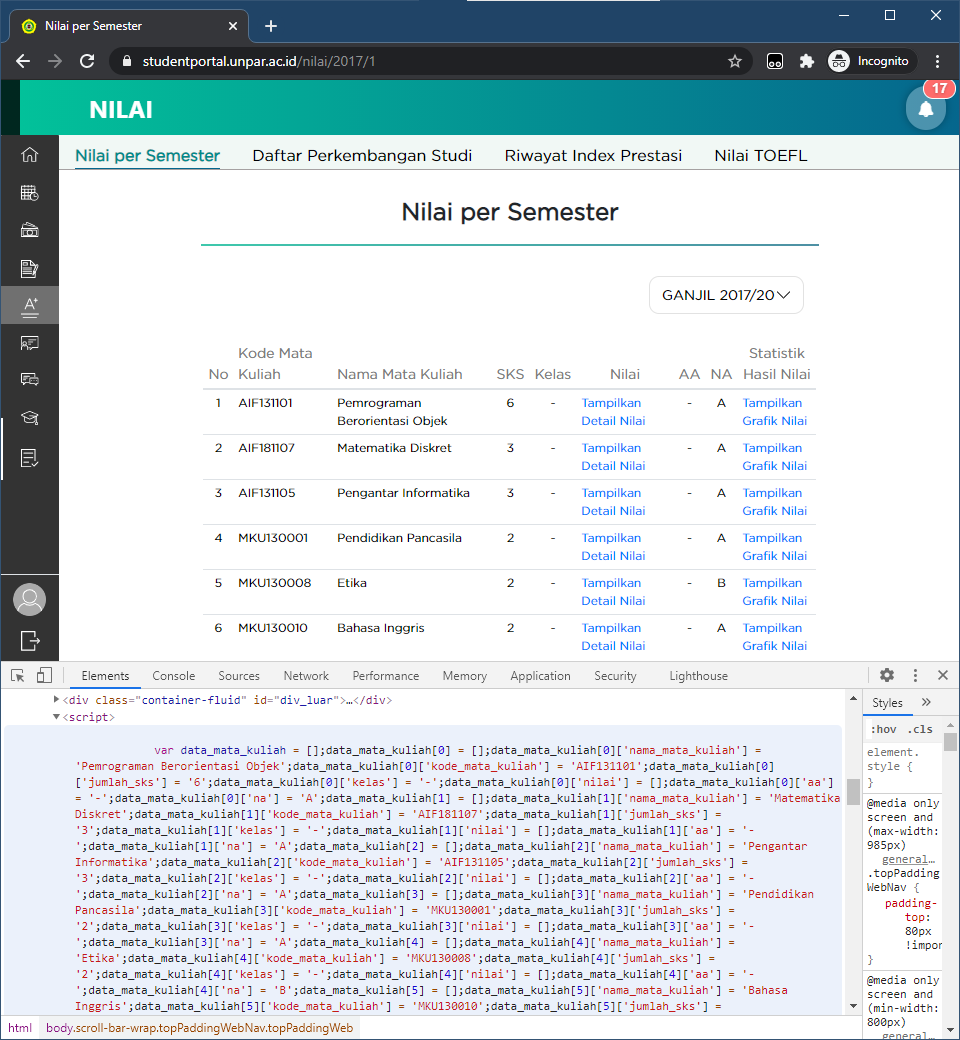
\includegraphics[scale=0.5]{Gambar/nilai_script.png}
        	\caption{\textit{Script} Data Nilai Mahasiswa Pada Halaman Nilai}
        	\label{fig:4_nilai_script}
        \end{figure}
	\end{itemize}
\end{enumerate}

Penjelasan mengenai kelas, \textit{method}, dan atribut pada \textit{package SIAKAD} adalah sebagai berikut:
\begin{enumerate}

\item{SIAkadDataPuller}\\
	Kelas ini merupakan turunan dari kelas \texttt{DataPuller} \ref{datapuller}. Kelas ini memiliki fungsi untuk mengambil username dan \textit{password} dosen yang disimpan dalam sebuah \textit{file}, dan kemudian memanggil \textit{method} pada kelas \texttt{SIAkad}. Atribut yang dimiliki kelas ini adalah sebagai berikut:
	\begin{itemize}
        \item \texttt{private final SIAkad siakad:} menyimpan objek \texttt{SIAkad}.
	\end{itemize}
	
	\textit{Method} yang dimiliki kelas ini adalah sebagai berikut:
	\begin{itemize}
		\item \texttt{public SIAkadDataPuller()}\\
		Berfungsi sebagai \textit{constructor} kelas \texttt{SIAkadDataPuller}.
		
		\item \texttt{public Mahasiswa[] pullMahasiswas()}\\
	    Berfungsi untuk memanggil \textit{method} \texttt{requestMahasiswaList} pada kelas \texttt{SIAkad}.\\
		\textbf{Kembalian:} \textit{array} yang berisi daftar mahasiswa yang diwalikan oleh dosen terlogin.
		
		\item \texttt{public Mahasiswa pullMahasiswaDetail()}\\
	    Berfungsi untuk memanggil \textit{method} \texttt{requestRiwayatNilai}, dan \texttt{requestDataDiri} pada kelas \texttt{SIAkad}.\\
		\textbf{Kembalian:} objek mahasiswa yang telah ditambahkan datanya dari pengambilan data di SIAKAD.
	\end{itemize}
	
\item{SIAkad}\\
Kelas ini memiliki fungsi untuk melakukan pengambilan data dari SIAKAD untuk kemudian diolah dan ditampilkan. Atribut yang dimiliki kelas ini adalah sebagai berikut:
	\begin{itemize}
        \item \texttt{protected static final String SIAKAD\_BASE\_URL:} menyimpan \textit{url} utama SIAKAD.
        \item \texttt{protected static final String SSO\_BASE\_URL:} menyimpan \textit{url} halaman \textit{login} \textit{Single Sign On}(SSO) UNPAR.
        \item \texttt{protected static final String MU\_BASE\_URL:} menyimpan \textit{url} MU UNPAR.
        \item \texttt{protected static final int DEFAULT\_TIMEOUT:} waktu \textit{timeout}.
        \item \texttt{protected final Logger logger:} 
        \item \texttt{public static final String[] MONTH\_NAMES:} menyimpan nama-nama bulan dalam bahasa Indonesia.
        \item \texttt{Token token:} menyimpan \textit{cookies} yang dapat digunakan untuk mengakses menu di SIAKAD.
    \end{itemize}
    
	\textit{Method} yang dimiliki kelas ini adalah sebagai berikut:
	\begin{itemize}
	    \item \texttt{public SIAkad()}\\
	    Berfungsi sebagai \textit{constructor} kelas \texttt{SIAkad}.
	    
	    \item \texttt{public SIAkad(boolean verbose)}\\
	    Berfungsi sebagai \textit{constructor} kelas \texttt{SIAkad}.\\
	    \textbf{Parameter:}
		\begin{itemize}
			\item \texttt{verbose:} 
		\end{itemize}
		
	    \item \texttt{public boolean login(String username, String password)}\\
	    Berfungsi untuk melakukan login ke SI Akademik. Semua transaksi lain harus diawali dengan login.\\
	    \textbf{Parameter:}
		\begin{itemize}
			\item \texttt{username:} username dosen.
			\item \texttt{password:} password dosen.
		\end{itemize}
        \textbf{Kembalian:} \textit{true} jika \textit{login} berhasil, \textit{false} jika \textit{username/password} salah.
        
        \item \texttt{public void logout()}\\
	    Berfungsi untuk melakukan \textit{logout} dari SIAKAD.
	    
	    \item \texttt{public List<Mahasiswa> requestMahasiswaList()}\\
	    Berfungsi untuk mendapatkan daftar mahasiswa yang diwalikan oleh dosen terlogin.\\
        \textbf{Kembalian:} daftar mahasiswa yang diwalikan oleh dosen terlogin.
        
        \item \texttt{public List<Mahasiswa> requestMahasiswaList(Set<ProgramStudi> programStudi, Mahasiswa.Status status, Integer angkatan)}\\
         Berfungsi untuk mendapatkan daftar mahasiswa yang diwalikan oleh dosen terlogin.\\
        \textbf{Parameter:}
		\begin{itemize}
			\item \texttt{programStudi:} program studi yang dipilih, atau null jika ingin mencari dari seluruh program studi yang terdaftar di SIAModels.
			\item \texttt{status:} status mahasiswa yang ingin ditampilkan, atau null jika default (aktif).
			\item \texttt{angkatan:} tahun angkatan, atau null jika semua.
		\end{itemize}
        \textbf{Kembalian:} daftar mahasiswa yang diwalikan oleh dosen terlogin.

	    \item \texttt{public Mahasiswa requestDataDiri(Mahasiswa mahasiswa)}\\
	    Berfungsi untuk mendapatkan data diri mahasiswa. Saat ini hanya mendukung \textit{URL} foto, tanggal lahir, dan jenis kelamin tanpa data diri yang lain.\\
	    \textbf{Parameter:}
		\begin{itemize}
			\item \texttt{mahasiswa:} mahasiswa yang ingin diperiksa.
		\end{itemize}
        \textbf{Kembalian:} objek mahasiswa yang sama, dengan data diri yang sudah dilengkapi.
        
        \item \texttt{public Mahasiswa requestRiwayatNilai(Mahasiswa mahasiswa, boolean includeLastSemester)}\\
        Berfungsi untuk mendapatkan daftar lengkap riwayat nilai mahasiswa, berdasarkan halaman "Data Akademik". Metode ini dapat mengisi lengkap kelas, nilai-nilai Tugas, UTS, UAS, serta NA.\\
        \textbf{Parameter:}
		\begin{itemize}
			\item \texttt{mahasiswa:} mahasiswa yang ingin diperiksa.
			\item \texttt{includeLastSemester:}apakah ingin mengikutsertakan nilai semester terakhir yang tercatat. Kelemahan metode "Data Akademik" adalah tidak bisa membedakan antara nilai yang belum rilis dengan yang sudah. Jika mahasiswa sedang menjalani mata kuliah tersebut, nilai sudah muncul tetapi kemungkinan NA nya berisi E karena nilai tugas/UTS/UAS belum lengkap. Jika mahasiswa sedang tidak menjalani kuliah tersebut (misal, saat FRS atau saat libur, maka nilai semester terakhir perlu diikutsertakan, karena mengacu ke nilai yang sudah rilis). Tentu saja ke depannya perlu mekanisme yang lebih baik yang dapat mendeteksi nilai yang sudah/belum rilis ini.
		\end{itemize}
        \textbf{Kembalian:} objek mahasiswa yang sama, dengan nilai yang sudah didapatkan (terurut secara kronologis dari yang paling lama ke baru).
        
        \item \texttt{protected Connection createBaseConnection(String url, Token token)}\\
        Berfungsi untuk membuat koneksi, dengan kondisi sudah melakukan \textit{login}.\\
        \textbf{Parameter:}
		\begin{itemize}
		    \item \texttt{url:} \textit{URL} yang dituju.
		    \item \texttt{token:} token autentikasi.
		\end{itemize}
        \textbf{Kembalian:} koneksi tersebut.

        \item \texttt{protected void logConnnection(Connection connection)}\\
        Berfungsi untuk memeriksa \textit{verbose flag}, dan apabila \textit{true}, akan menampilkan \textit{debug output}.\\
        \textbf{Parameter:}
		\begin{itemize}
		    \item \texttt{connection:} \textit{connection request} dan \textit{response}.
		\end{itemize}
	\end{itemize}
    
\item{Token}\\
Kelas ini memiliki fungsi untuk menyimpan \textit{cookies}. Atribut yang dimiliki kelas ini adalah sebagai berikut:
	\begin{itemize}
        \item \texttt{private final Map<String, String> cookies:} menyimpan \textit{cookies}.
	\end{itemize}
	
	\textit{Method} yang dimiliki kelas ini adalah sebagai berikut:
	\begin{itemize}
	    \item \texttt{public Token(Map<String, String> cookies)}\\
	    Berfungsi sebagai \textit{constructor} kelas \texttt{Token}.
	    
	    \item \texttt{public Map<String, String> getCookies()}\\
	    Berfungsi untuk mendapatkan \textit{cookies}.\\
        \textbf{Kembalian:} \textit{cookies}.
        
        \item \texttt{public void injectToConnection(Connection connection)}
        Berfungsi untuk memasukkan \textit{session} ke dalam \textit{connection}.\\
        \textbf{Parameter:}
		\begin{itemize}
		    \item \texttt{connection:} koneksi yang ingin dimasukkan \textit{session}.
		\end{itemize}
    \end{itemize}
\end{enumerate}

\section{Perancangan Antarmuka}
Gambar \ref{fig:4_antarmuka} menunjukkan rancangan antarmuka dari aplikasi \textit{screensaver}. Antarmuka aplikasi akan menampilkan foto dari mahasiswa apabila foto tersebut tersedia. Baris pertama merupakan nama dari mahasiswa, kemudian baris kedua akan diisi oleh angkatan dari mahasiswa tersebut. Baris ketiga menampilkan usia dan tanggal lahir mahasiswa. Baris keempat merupakan status dari mahasiswa tersebut apabila tersedia. Baris kelima merupakan \textit{email} mahasiswa dimana format \textit{email} mahasiswa UNPAR adalah \textbf{NomorPokokMahasiswa@student.unpar.ac.id}. Baris keenam berisi nilai TOEFL terakhir mahasiswa apabila mahasiswa tersebut sudah mengambil ujian TOEFL, atau diisi "Tidak Tersedia" apabila mahasiswa tersebut belum mengambil ujian TOEFL. Baris ketujuh menampilkan IPS dan IPK dari mahasiswa tersebut. Baris terakhir diisi oleh jumlah sks yang telah lulus dan jumlah sks yang telah ditempuh oleh mahasiswa tersebut. Setiap 5 detik tampilan aplikasi akan berubah ke mahasiswa berikutnya. Namun pada aplikasi yang dibuat oleh terbimbing, data yang ditampilkan hanya mahasiswa itu sendiri, sedangkan pada aplikasi yang dibuat oleh pembimbing, data yang ditampilkan akan berubah.
\begin{figure}[H]
	\centering
	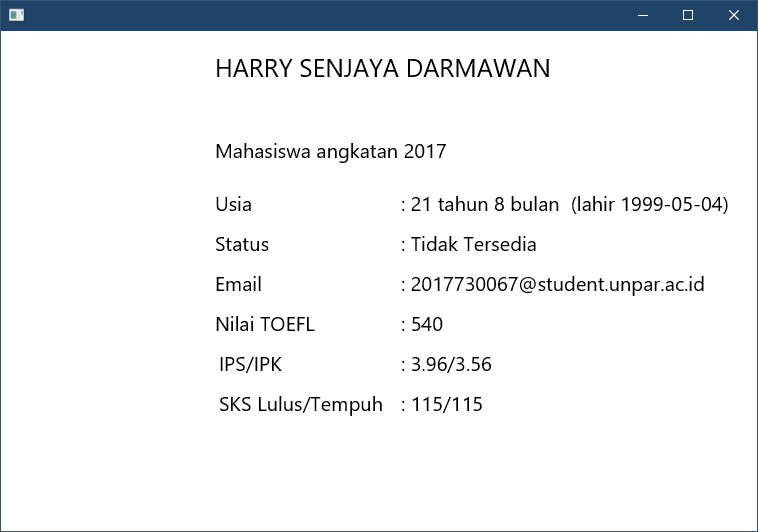
\includegraphics[scale=0.5]{Gambar/UI.png}
	\caption{Rancangan Antarmuka \textit{Screensaver}}
	\label{fig:4_antarmuka}
\end{figure}

\begin{figure}[H]
	\centering
	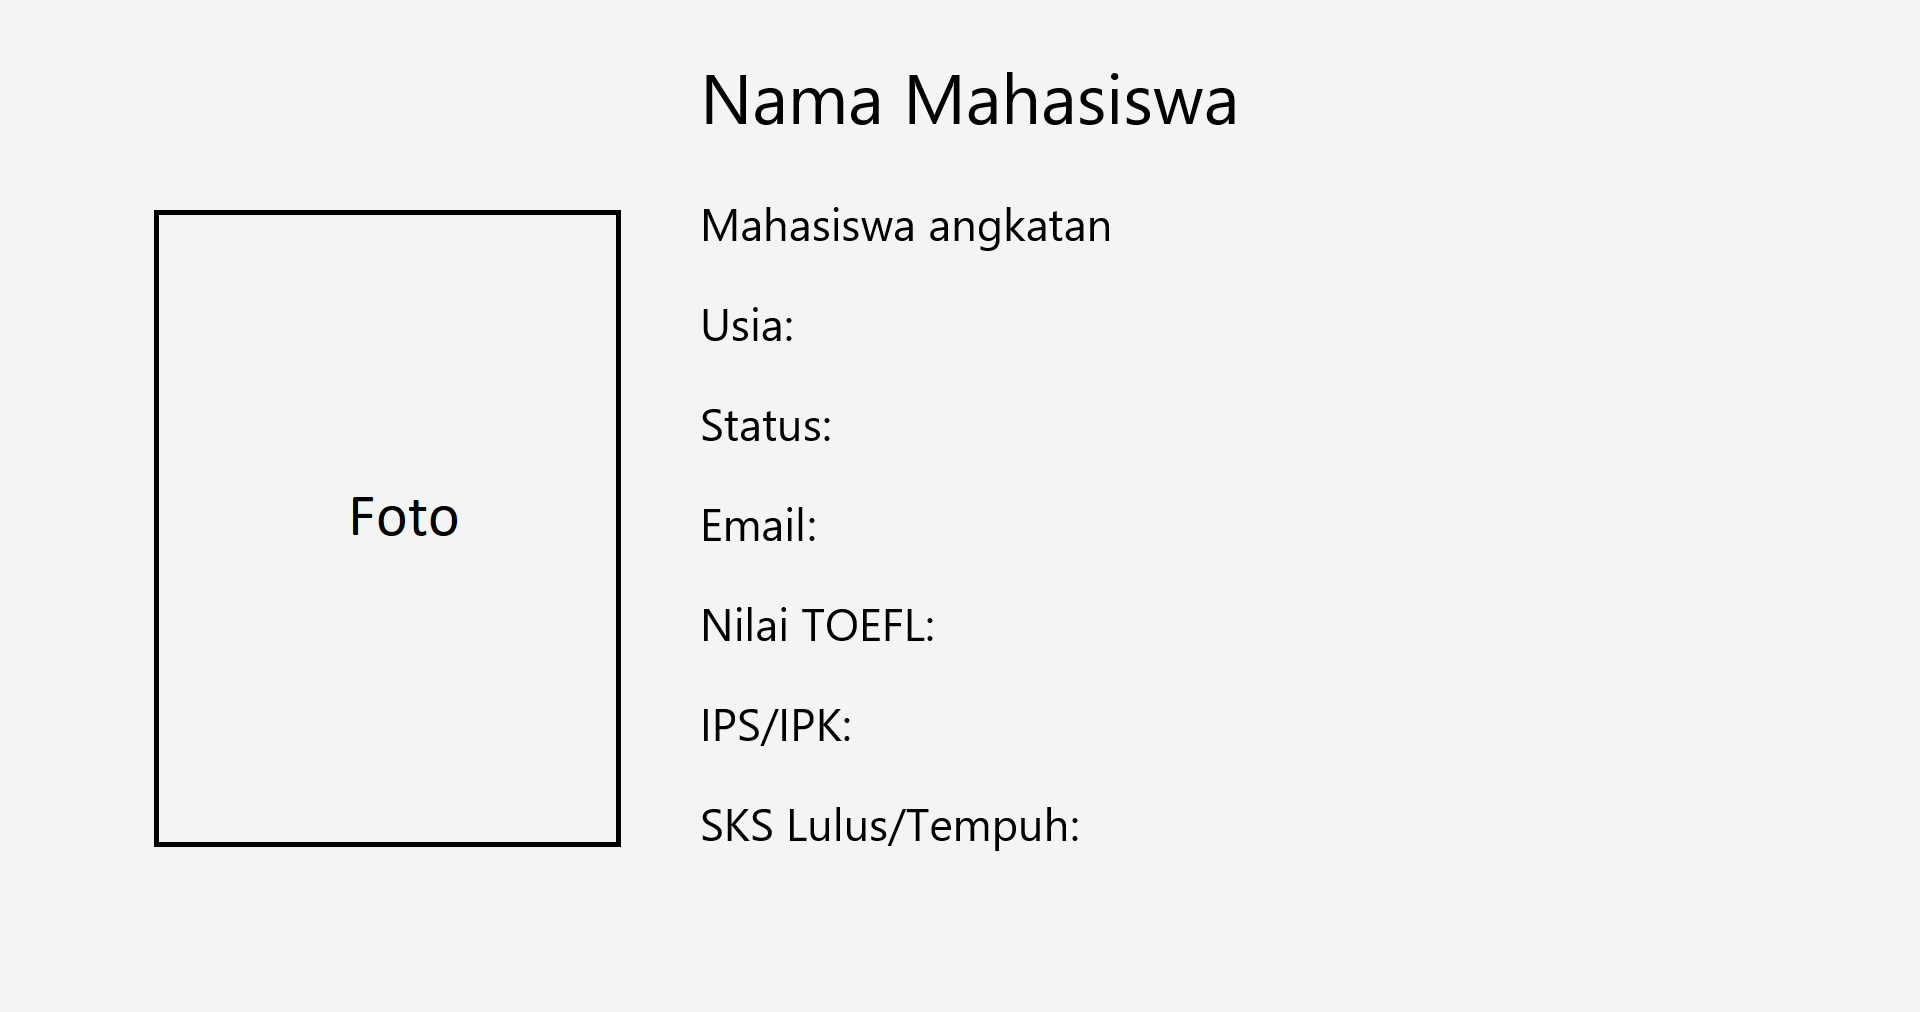
\includegraphics[scale=0.2]{Gambar/UI2.png}
	\caption{Rancangan Antarmuka \textit{Screensaver}}
	\label{fig:4_antarmuka}
\end{figure}